\tocless\subsection{Objective}
As seen in the last experiment, it is possible that colour plays a significant part in the overall classification of some food types, along with shape and texture. Due to this, what would happen if colour was removed from the image? The three images, Figure \ref{fig:bananaPreRes}, Figure \ref{fig:apple_piePreRes} and Figure \ref{fig:pizzaPreRes}, were all converted to greyscale to test this and the resulting images can be seen in Figure \ref{fig:bananaGrey}, Figure \ref{fig:applePieGrey} and Figure \ref{fig:pizzaGrey}. Each of these images were ran through the model before and after converting to greyscale and the results recorded.

\begin{figure}[h]
	\centering
    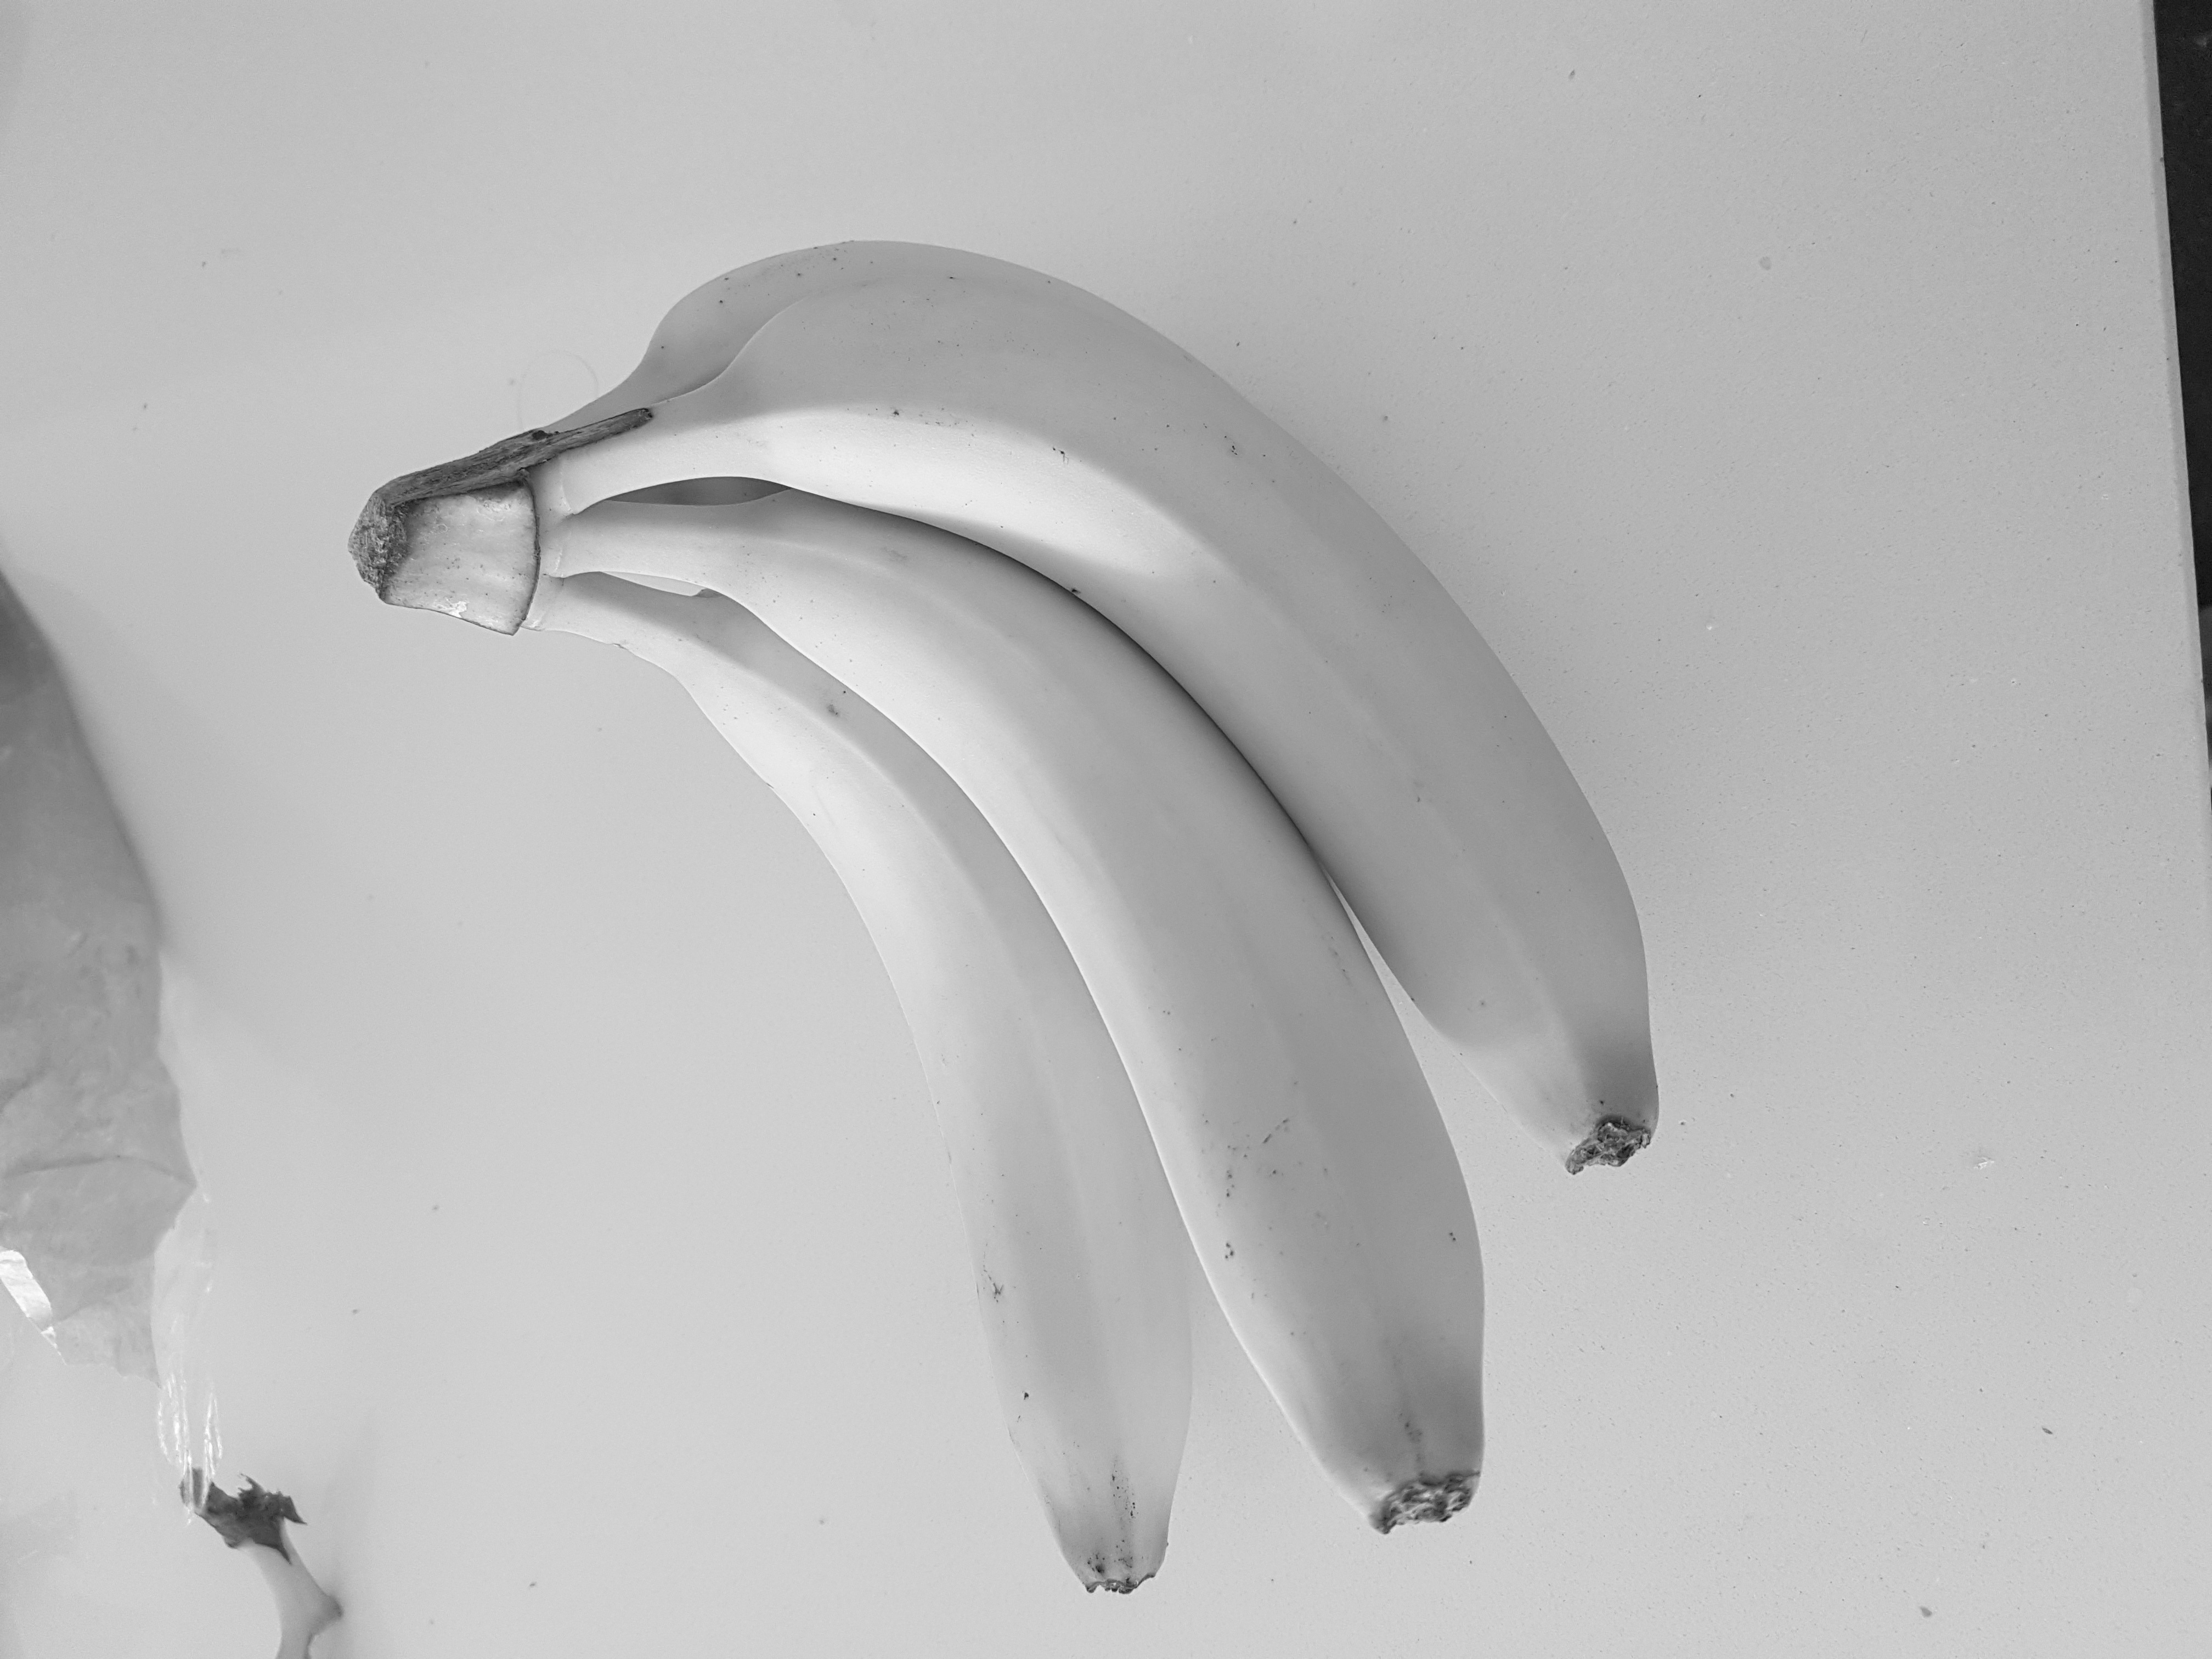
\includegraphics[scale=0.05]{banana_grey}
    \caption{Banana Image Greyscale}
    \label{fig:bananaGrey}
\end{figure}

\begin{figure}[h]
	\centering
    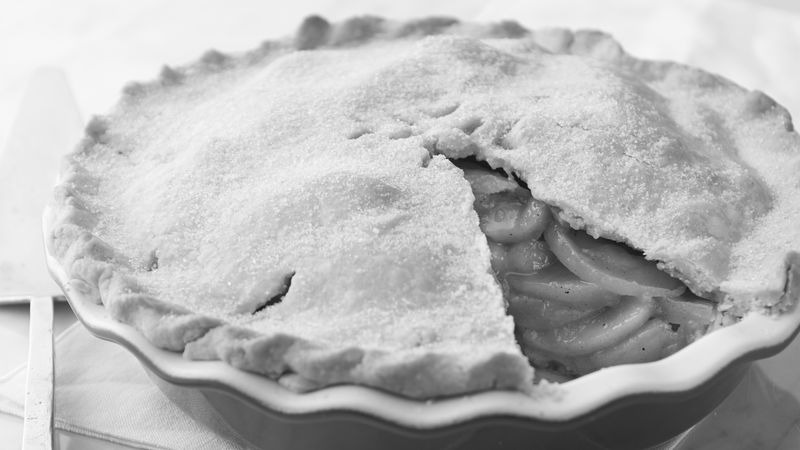
\includegraphics[scale=0.25]{pie_grey}
    \caption{Apple Pie Image Greyscale}
    \label{fig:applePieGrey}
\end{figure}

\begin{figure}[h]
	\centering
    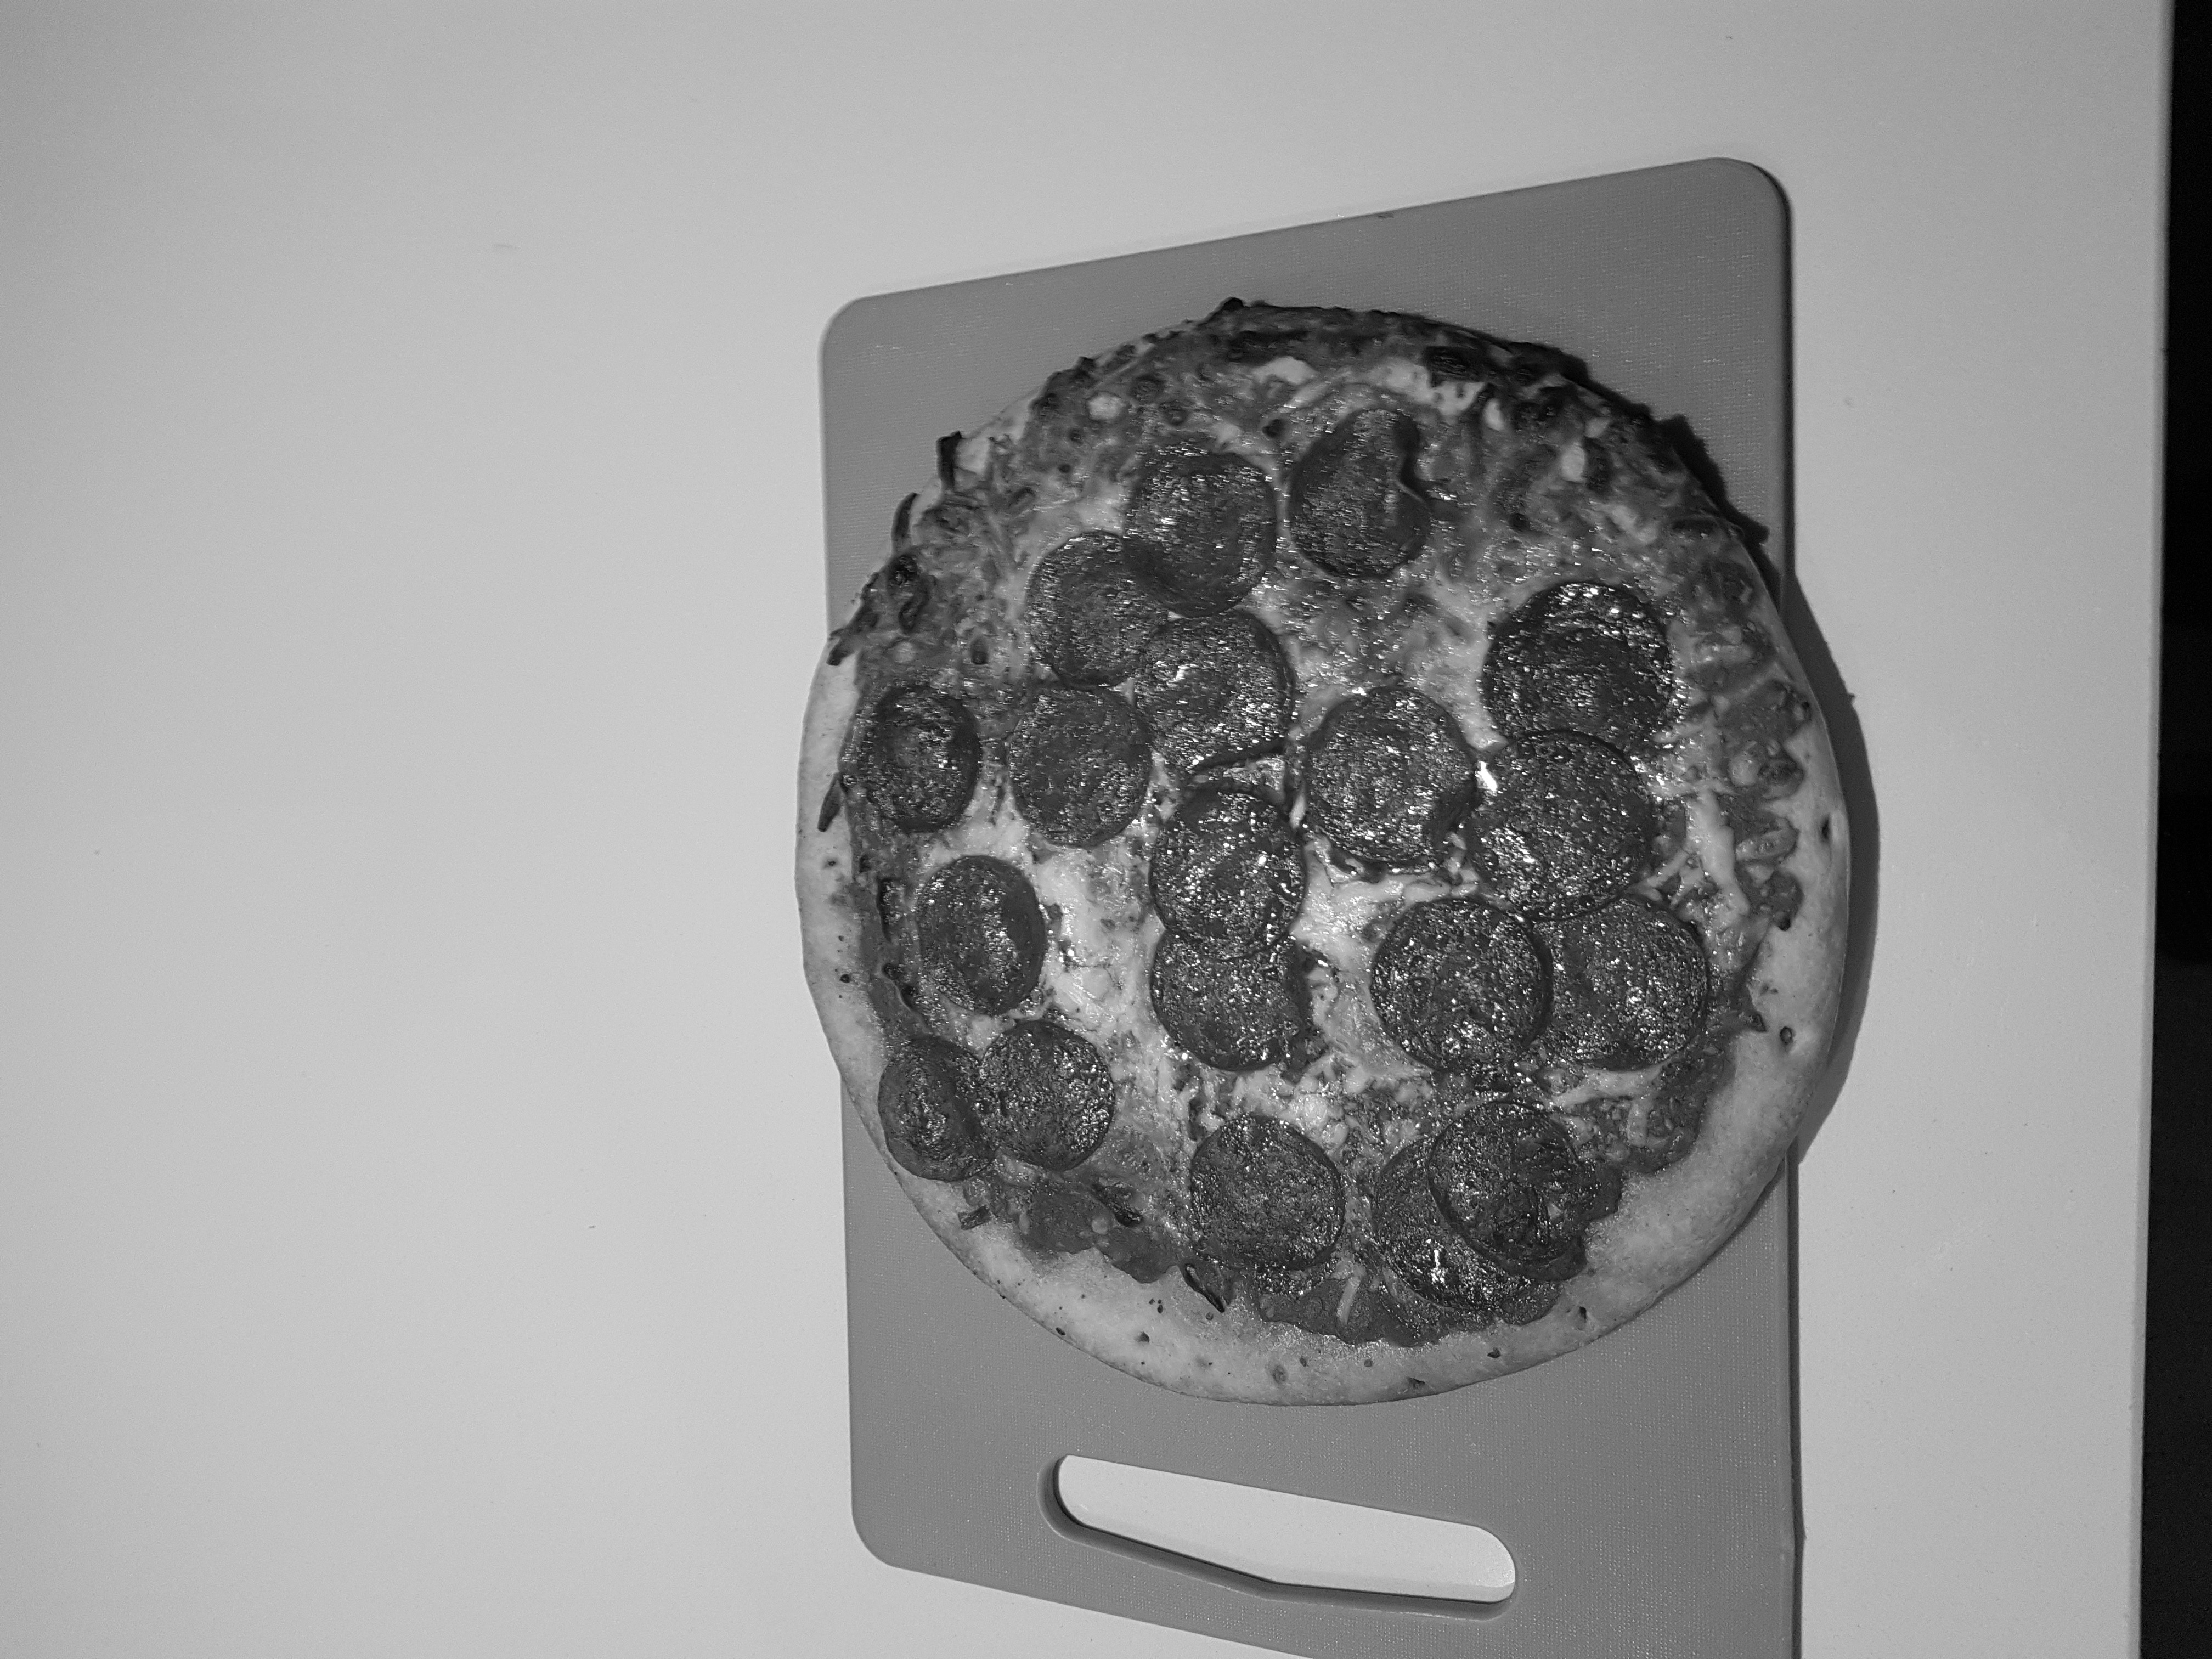
\includegraphics[scale=0.05]{pizza_grey}
    \caption{Pizza Image Greyscale}
    \label{fig:pizzaGrey}
\end{figure}

\tocless\subsection{Network Architecture}
Inception V-3 architecture. Parameter tuned model was used for this experiment.

\tocless\subsection{Dataset}
Food-101 extended dataset.

\tocless\subsection{Results}
The results for this experiment can be seen in Table \ref{colour}.
The 'Top 1' notation in the table suggests that the food was predicted as the number one prediction. The decimal value is the probability of that food type being the correct classification.

\begin{table}[]
\centering
\caption{Effect of Colour}
\label{colour}
\begin{tabular}{|l|l|l|}
\hline
\textbf{Food Image} & \textbf{Pre-Scaled Image} & \textbf{Greyscale}      \\ \hline
Banana     & Top 1 : 0.9971   & Top 1 : 0.9986 \\ \hline
Apple Pie  & Top 1 : 0.7986   & Top 1 : 0.3462   \\ \hline
Pizza      & Top 1 : 0.9753   & Top 2 : 0.1299 \\ \hline
\end{tabular}
\end{table}

\tocless\subsection{Analysis}
\tocless\subsubsection{Colour}
In regard to the images of the banana (Figure \ref{fig:bananaPreRes} and Figure \ref{fig:bananaGrey}), there is very little difference in classification. They were both classified to a Top 1 accuracy and their probabilities differing by only 0.0015 with the grey scale image being of a higher probability. This would indicate that colour is not an important factor for classifying bananas and the coloured image may even have noise. This can be seen in Table \ref{colour}.

The apple pie images (Figure \ref{fig:apple_piePreRes} and Figure \ref{fig:applePieGrey}) were also both classified correctly but with a large gap in the likelihood of that classification being correct. As per Table \ref{colour}, the coloured image had a probability of 0.7986 as opposed to one of 0.3462. This would indicate that while colour is important, there is enough unique data from the rest of the image to result in correct classification.

Finally, the pizza images (Figure \ref{fig:pizzaPreRes} and Figure \ref{fig:pizzaGrey})were the most contrasting in their results. While the original image was classified to Top 1 accuracy with a likelihood of 0.9753, the coloured image was classified to Top 2 accuracy while a probability of 0.1299. From this we can deduce that colour is vital for the classification of pizza.

Since this experiment only compared three images, we cannot say for sure if this analysis is biased or not.

\tocless\subsubsection{Colour vs Scale}
In the last experiment, it was seen that the pizza and banana images (Figure \ref{fig:pizzaPreRes} and Figure \ref{fig:bananaPreRes}) were not really affected by image quality. While this seems to be true, the image of apple pie, Figure \ref{fig:apple_piePreRes}, was greatly influenced by only being classified to a Top 5 accuracy when down scaled.

For the greyscale images, bananas were not affected greatly and neither was an apple pie but a pizza was greatly influenced.

From this, the prominent unique features for each of these food types are different. The banana (Figure \ref{fig:bananaPreRes}) may have focus on shape and texture, the pie (Figure \ref{fig:apple_piePreRes}) on image quality and some influence of colour while the pizza (Figure \ref{fig:pizzaPreRes}) may have a focus on shape, texture and colour.

